This section provides some useful benchmarking of the final eKwip prototype to ensure the accuracy and precision of the collected measurements are comparable to industry standards. The performance of the wrap is then assessed against the accuracy and precision required to determine the risk of ACL injuries. Finally, some sample data collected by eKwip on healthy and injured patients is shown at the end of the section.

\subsection {Performance}
In order to correctly predict ACL injuries in real time, data must be collected at a certain frequency so that subtle movements and accelerations are captured in the data. Data transfer speeds were a major concern throughout work on the project. Problems with the library used in data transfer were identified and rectified, allowing eKwip to trasmit the movements and acceleration data at useful speeds.

Another issue with performance resulted from the WiFi module buffering data until the data packet was large enough to send.  Configuring the WiFi module to send data after receipt of each data packet as well as shortening the data string used to communicate each data point further increased transmission speed. These changes sped up the data presented on the server by about 14.5\%, a major increase and critical for the different use cases of eKwip. 

The improvements in data sampling and network transmission rates can be seen in Figure~\ref{fig:graph}.

\begin{figure}[h]
  \begin{center}
    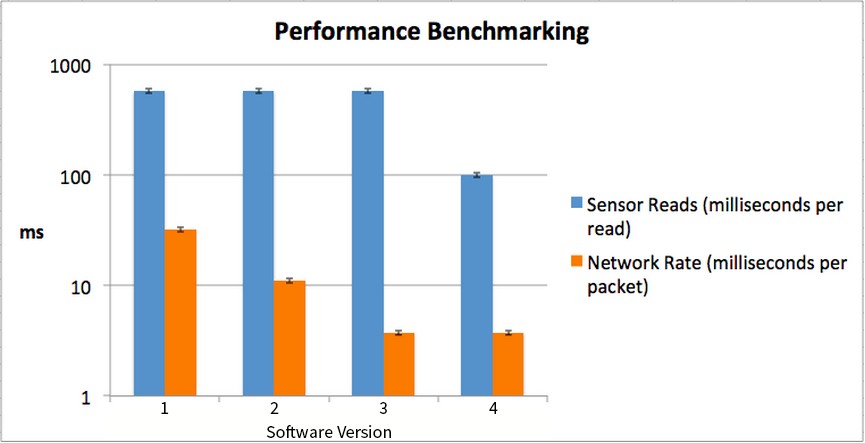
\includegraphics[width=3in]{images/graph.png}
  \end{center}
  \caption{Network and sensor performance of eKwip in various versions}
  \label{fig:graph}
\end{figure}


The accuracy of eKwip is determined by measuring the actual angle of the knee and comparing it to the angle given by the sensors. The final prototype scored an error of 5.00\% with a standard deviation of 3.39\%. This is compared to the KT1000, the current standard of measuring flexion angles in physical therapy. The KT1000 has an error of about 1.89\% and standard deviation of 2.50\% "!!!! THE KT1000 reference". While the KT1000 is more precise, it is also more bulky. By using eKwip, physical therapists can use a less obstrusive device on their patients.

Proximity of the sensors to the leg is also important in producing an accurate measurement of the movements of the wearer. The proximity is measured from various knee positions of the wearer to the skin of the upper and lower leg. The average distance from the sensors are found to be 0.22cm with a standard deviation of 0.08cm. 

The precision of eKwip is determined by repeated measurements of the same position of the knee, confirmed by a protractor. The average standard deviation of eKwip is found to be 1.05\%.

\subsection {Testing eKwip}
Two subjects were used in testing out eKwip's accuracy and measuring capabilities: Subject A, who suffered no knee injury, and Subject B, who had recently recovered from an ACL injury. The wrap was not tested on both knees of the injured subject due to the possibility that the healthy knee of the subject may compensate for the injured knee, skewing any data collected. Both subjects wore the wrap on the right knee (which was the injured knee for our injured subject) and walked on a treadmill for 10 seconds.

The data collected and saved on our server was used to calculate the knee flexion angles of both subjects "!!!! WE MAY NEED TO DISCUSS HOW WE CAME UP WITH THE ANGLES". As seen in Figure~\ref{fig:results_graph}, there is a clear difference in the flexion angles of the healthy subject compared to the unhealthy subject. The flexion angles of Subject A was 3 \pm 1.5 degrees. This is compared to Subject B, whose flexion angles were about 5 \pm 3 degrees. The flexion angles of Subject B varied far greater and remained close to the dangerous angle zone of 6-8 degrees. Through the data, eKwip's monitoring and measuring capabilties were verified to detect a clear difference between a health and injured subject.


\begin{figure}[h]
  \begin{center}
    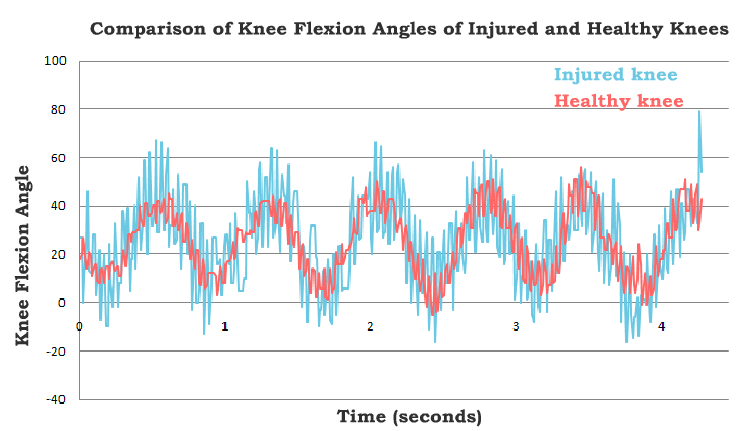
\includegraphics[width=3.4in]{images/results_graph.PNG}
  \end{center}
  \caption{Block diagram of eKwip system}
  \label{fig:results_graph}
\end{figure}